%%%%%%%%%%%%%%%%%%%%%%%%%%%%%%%%%%%%%%%%%
% Beamer Presentation
% LaTeX Template
% Version 1.0 (10/11/12)
%
% This template has been downloaded from:
% http://www.LaTeXTemplates.com
%
% License:
% CC BY-NC-SA 3.0 (http://creativecommons.org/licenses/by-nc-sa/3.0/)
%
%%%%%%%%%%%%%%%%%%%%%%%%%%%%%%%%%%%%%%%%%

%----------------------------------------------------------------------------------------
%	PACKAGES AND THEMES
%----------------------------------------------------------------------------------------

\documentclass{beamer}

\mode<presentation> {

% The Beamer class comes with a number of default slide themes
% which change the colors and layouts of slides. Below this is a list
% of all the themes, uncomment each in turn to see what they look like.

%\usetheme{default} % +
%\usetheme{AnnArbor}
%\usetheme{Antibes}
%\usetheme{Bergen}
%\usetheme{Berkeley} % +
%\usetheme{Berlin}
%\usetheme{Boadilla} % +
%\usetheme{CambridgeUS}
%\usetheme{Copenhagen}
%\usetheme{Darmstadt}
%\usetheme{Dresden} 
%\usetheme{Frankfurt} % +
%\usetheme{Goettingen}
%\usetheme{Hannover}
%\usetheme{Ilmenau}
%\usetheme{JuanLesPins}
%\usetheme{Luebeck}
%\usetheme{Madrid} % +
%\usetheme{Malmoe}
%\usetheme{Marburg}
%\usetheme{Montpellier}
%\usetheme{PaloAlto}
%\usetheme{Pittsburgh}
%\usetheme{Rochester}
\usetheme{Singapore} % +
%\usetheme{Szeged}
%\usetheme{Warsaw}

% As well as themes, the Beamer class has a number of color themes
% for any slide theme. Uncomment each of these in turn to see how it
% changes the colors of your current slide theme.

%\usecolortheme{albatross}
%\usecolortheme{beaver}
%\usecolortheme{beetle}
%\usecolortheme{crane}
%\usecolortheme{dolphin}
%\usecolortheme{dove}
%\usecolortheme{fly}
%\usecolortheme{lily}
%\usecolortheme{orchid}
%\usecolortheme{rose}
%\usecolortheme{seagull}
%\usecolortheme{seahorse}
%\usecolortheme{whale}
%\usecolortheme{wolverine}

%\setbeamertemplate{footline} % To remove the footer line in all slides uncomment this line
%\setbeamertemplate{footline}[page number] % To replace the footer line in all slides with a simple slide count uncomment this line

%\setbeamertemplate{navigation symbols}{} % To remove the navigation symbols from the bottom of all slides uncomment this line
}


\logo{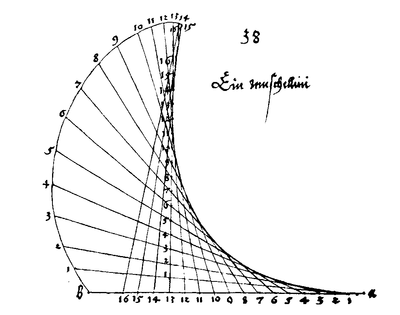
\includegraphics[height=1cm]{./images/logo.png}}


\usepackage{graphicx} % Allows including images
\usepackage{booktabs} % Allows the use of \toprule, \midrule and \bottomrule in tables
\usepackage{caption}
\usepackage{subcaption}
\usepackage{array}
%\usepackage{tcolorbox}

%----------------------------------------------------------------------------------------
%	TITLE PAGE
%----------------------------------------------------------------------------------------

\title[Epidemics Wokrshop]{G-CSC Epidemics\newline Disease modelling via SEIRD}

\author{\textcolor{blue}{Yannick Rosam\\}}
\institute[G-CSC] % Your institution as it will appear on the bottom of every slide, may be shorthand to save space
{
Goethe Universtiy Frankfurt - Center for Scientific Computing \\ % Your institution for the title page
\medskip
%\textit{john@smith.com} % Your email address
}
%\date{\today} % Date, can be changed to a custom date

\begin{document}

%----------------------------------------------------------------------------------------
%	PRESENTATION SLIDES
%----------------------------------------------------------------------------------------


\begin{frame}
\titlepage % Print the title page as the first slide
\end{frame}

%----------------------------------------------------------------------------------------

\begin{frame}
\frametitle{Overview} 
\tableofcontents 
\end{frame}

%----------------------------------------------------------------------------------------
%	SECTION FORMATING
%----------------------------------------------------------------------------------------

%\AtBeginSection[]{
%  \begin{frame}
%  \vfill
%  \centering
%  \begin{beamercolorbox}[sep=8pt,center,shadow=true,rounded=true]{title}
%    \usebeamerfont{title}\insertsectionhead\par%
%  \end{beamercolorbox}
%  \vfill
%  \end{frame}
%}

%----------------------------------------------------------------------------------------
\section{Epidemics}
\subsection{Background}

\begin{frame}
	\frametitle{Basic Idea}
	\textbf{Concept:}
	\begin{enumerate}[$\bullet$]
		\item Modelling of diseases via differential equations
		\item Covid-19 as example disease\\
	\end{enumerate}
	\textit{ }\newline
	\textbf{Goal:} Establish model to predict future infection spreading using present day data\newline
	
	\textbf{Challanges:}
	\begin{enumerate}[$\bullet$]
		\item Data acquisition and preparation
		\item Definition of accurate assumptions\\
			(real life infection spreading and documentations is messy. So are gov. reactions)
		\item Finding parameters that accuratly predict the behaviour of the disease
	\end{enumerate}

\end{frame}

\begin{frame}
	\frametitle{Modelling}
	\textbf{Goal:} Model the spread of a disease
	\begin{enumerate}[$\bullet$]
		\item Most basic model: SIR (\textcolor{red}{S}usceptible, \textcolor{red}{I}nfected, \textcolor{red}{R}emoved)\\
	\end{enumerate}
	
	\textbf{add SIR image between bulletpoints}
	\begin{center}
		
\includegraphics[width=0.6\textwidth]{./images/SIRv2.png} %add SIR model image
	\end{center}
	\begin{enumerate}[$\bullet$]
		\item A given population "flows" from state to state
		\item This process can be used to describe a Pandemic/Epidemic 
		\item Questions involve:\\
			- How long does the Pandemic/Epidemic lasts?\\
			- How many people are infected at peak times?\\
			- What percentage of the population need to be immune for the spreading to stop?
	\end{enumerate}
\end{frame}

\begin{frame}
	\frametitle{Modelling}
		Many different types of model exist, we are working on SEIRD\newline
	\begin{enumerate}
		\item[\textcolor{red}{S}] Suceptible: At risk of contracting the disease
		\item[\textcolor{red}{E}] Exposed: Infected, but currently no symptoms
		\item[\textcolor{red}{I}] Infected: Fully infected, with symptoms
		\item[\textcolor{red}{R}] Recovered: Recovered from disease and immune to infection
		\item[\textcolor{red}{D}] Diceased: Died during the infection
	\end{enumerate}
	\vspace{0.1cm}
		\only<1>{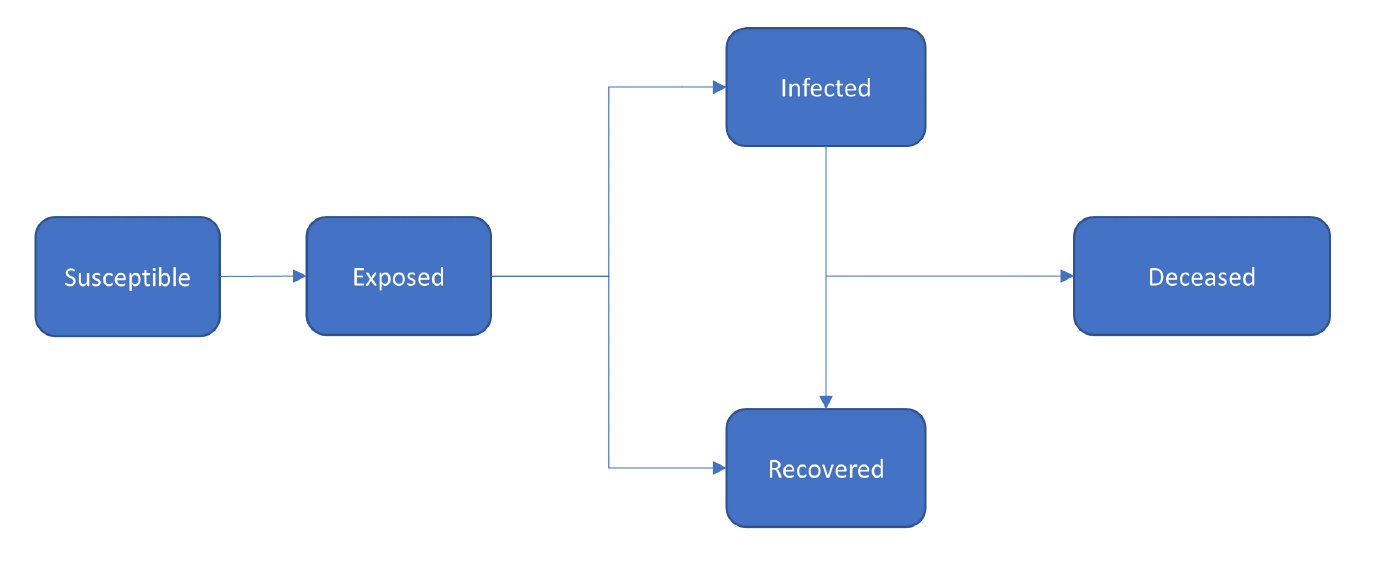
\includegraphics[height=0.3\textwidth]{./images/SEIRDv20.png}}
		\only<2>{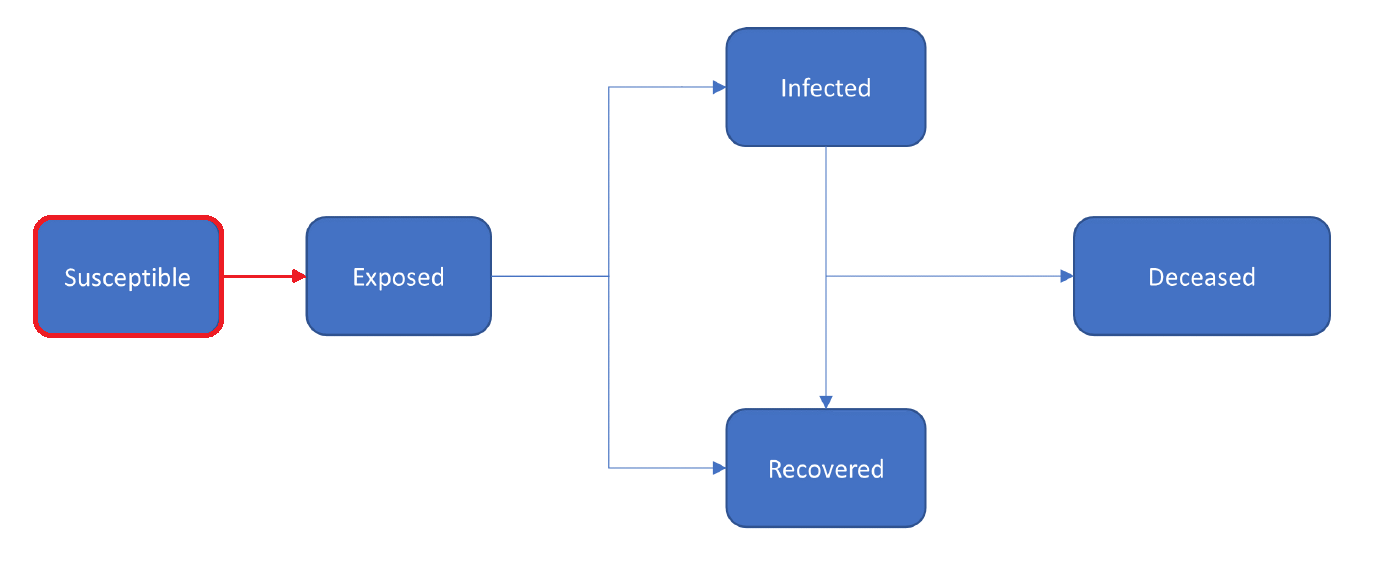
\includegraphics[height=0.3\textwidth]{./images/SEIRDv21S.png}}
		\only<3>{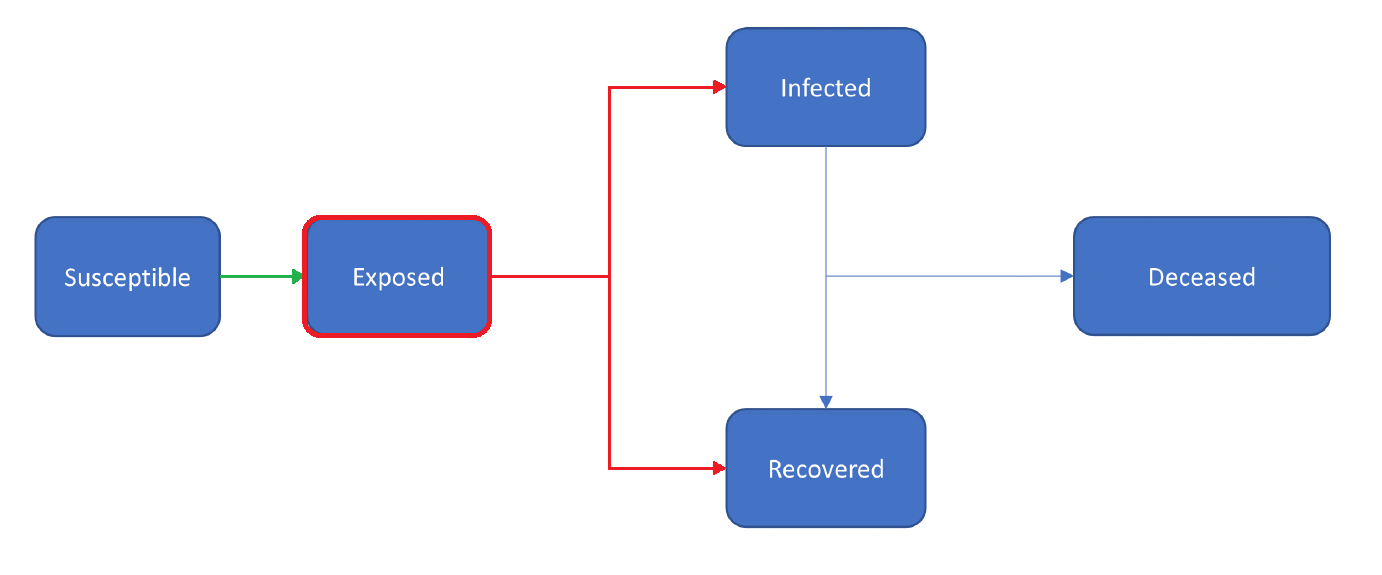
\includegraphics[height=0.3\textwidth]{./images/SEIRDv22E.png}}
		\only<4>{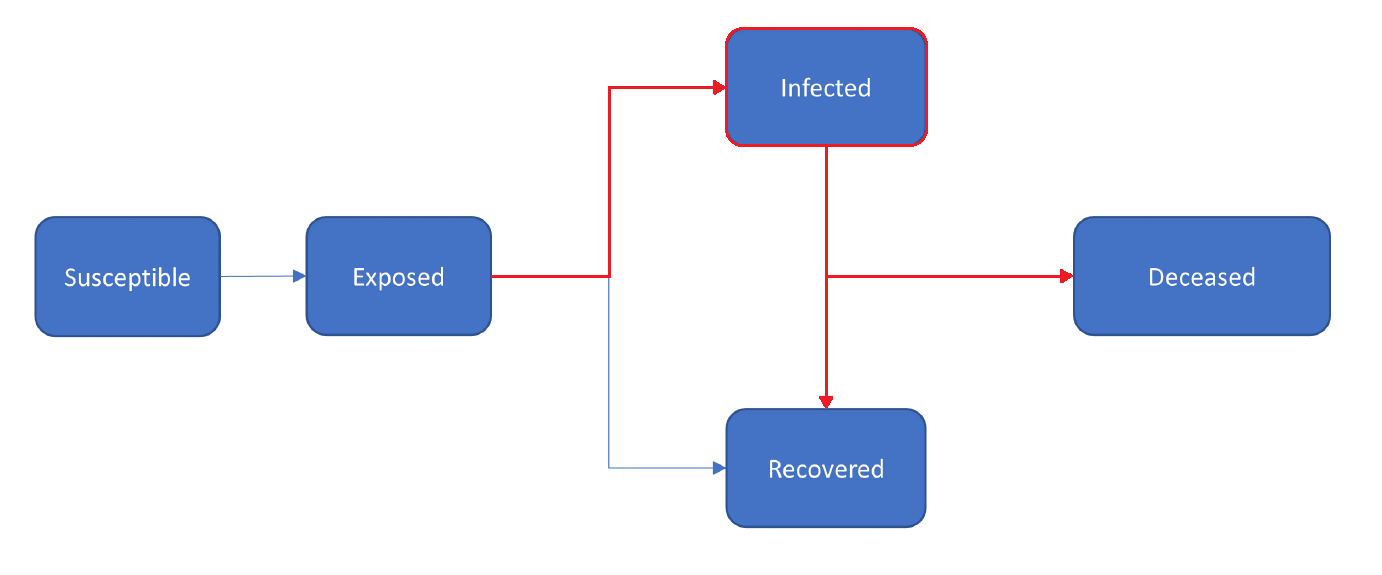
\includegraphics[height=0.3\textwidth]{./images/SEIRDv23I.png}}
		\only<5>{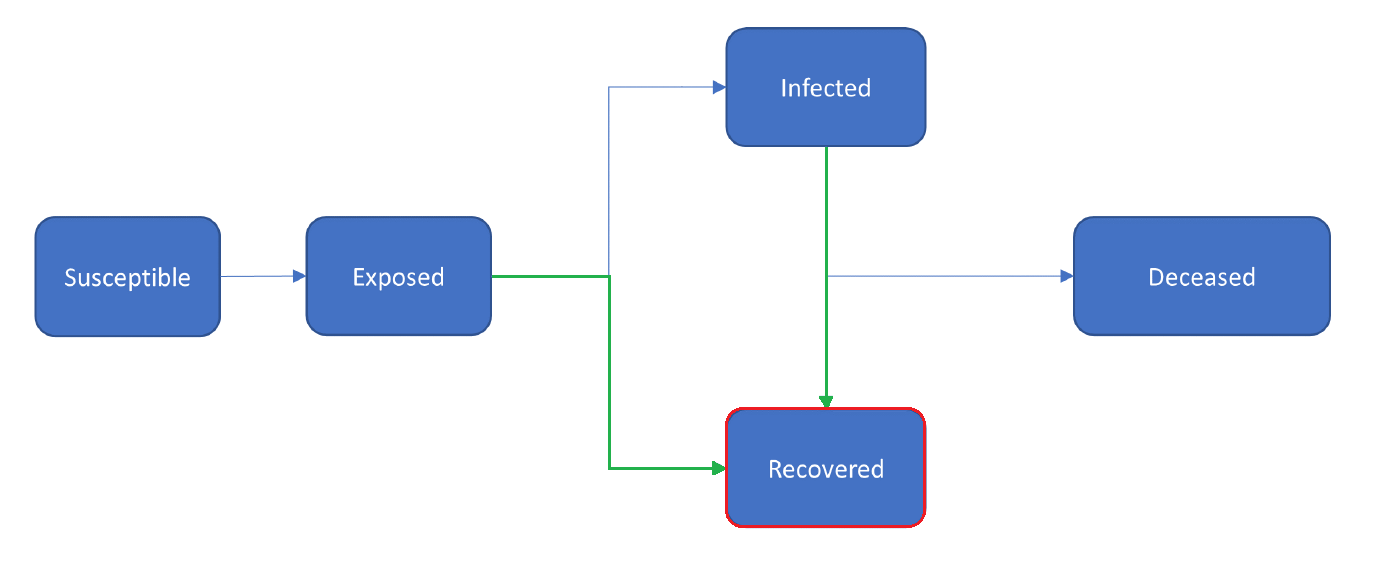
\includegraphics[height=0.3\textwidth]{./images/SEIRDv24R.png}}
		\only<6>{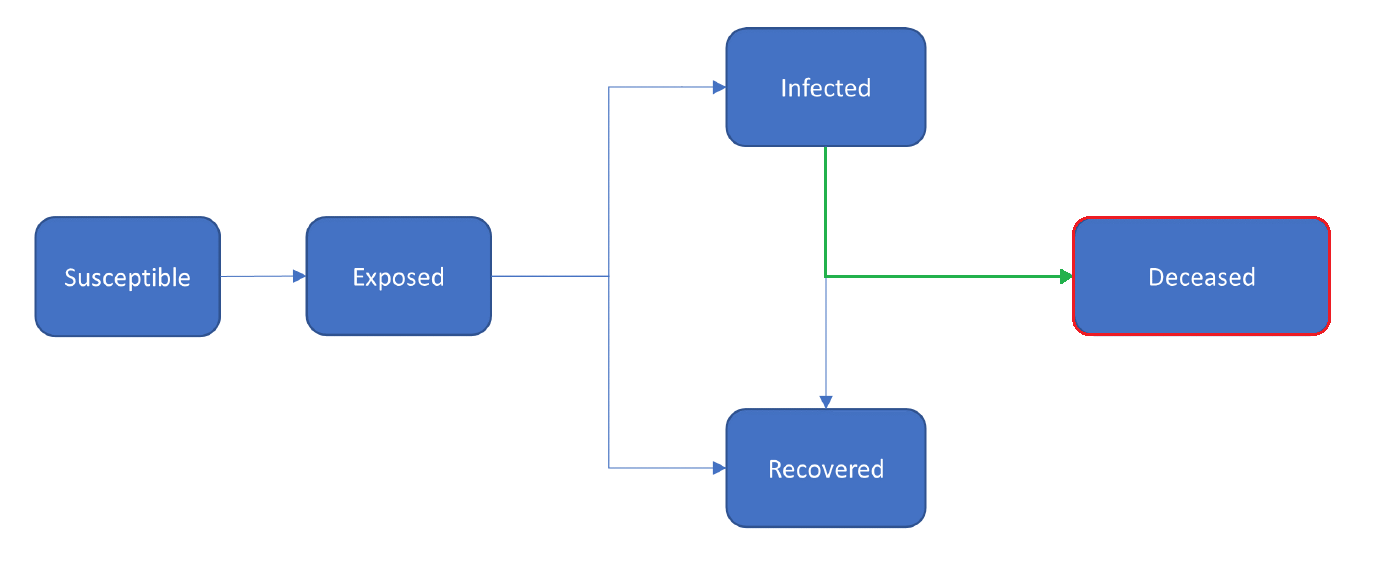
\includegraphics[height=0.3\textwidth]{./images/SEIRDv25D.png}}
\end{frame}

\begin{frame}
	\frametitle{Modelling}
	Modelling can be done using both:
	\begin{enumerate}[$\bullet$]
		\item ODE (\textcolor{red}{O}rdinary \textcolor{red}{D}ifferntial \textcolor{red}{E}quations)
		\item PDE (\textcolor{red}{P}artial \textcolor{red}{D}ifferentical \textcolor{red}{E}quations)
	\end{enumerate}
	\textit{ }\newline
	In the context of Epidemics:
	\begin{enumerate}[$\bullet$]
		\item ODE: Simulate disease spreading for a single location (time dependency)
		\item PDE: Simulate disease dependent of time and other variables (location, demographic, etc.) 
	\end{enumerate}
	\textit{ }\newline
	We currently focus on PDE simulation using grids of germany (time, location dependent)
\end{frame}

%----------------------------------------------------------------------------------------

\subsection{Project state}

\begin{frame}
\frametitle{Accomplishments}
	\begin{enumerate}[$\bullet$]
		\item Tristan and Devansh build a code base for the project
		\item Devansh tested and optimized the PDE model for seven big cities in germany
		\item The entire team helped to build, maintain and evlolve a GUI for (on demand) disease simulation [ongoing]
	\end{enumerate}
\end{frame}

%----------------------------------------------------------------------------------------

\subsection{Currently in progress}

\begin{frame}
\frametitle{The GUI - EpidemicsRunner} 
	\textbf{Features:}
	\begin{enumerate}[$\bullet$]
		\item ODE and PDE simulation
		\item Parameter optimization using different algorithms and ConstrainedOptimization (\textit{Scheidemann et al.})
	\end{enumerate}

	\textbf{Upcoming:}
	\begin{enumerate}[$\bullet$]
		\item User gets to choose between implicit and explicit solver
		\item Performace improvement of implicit solver
		\item Integrate grid definition into GUI [optional]
	\end{enumerate}
\end{frame}

\begin{frame}
\frametitle{Hessen model} 
	\textbf{Current goals:}
	\begin{enumerate}[$\bullet$]
		\item Establish PDE model with interconnected regions [done]
		\item Optimize parameters and try to replicate real live data\newline [in progress]
		\item Check howdiffusion between regions improves the model
	\end{enumerate}
	\begin{figure}
		\centering
		\begin{subfigure}[b]{0.45\textwidth}
			\centering
			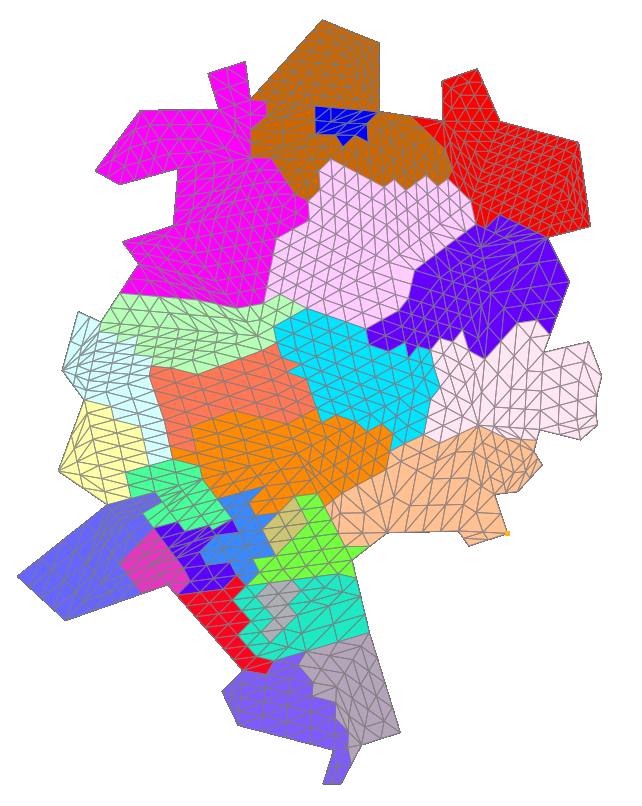
\includegraphics[height=3.5cm]{./images/mesh2.png}
			\caption*{Hessen grid}
		\end{subfigure}
		\begin{subfigure}[b]{0.45\textwidth}
			\centering
			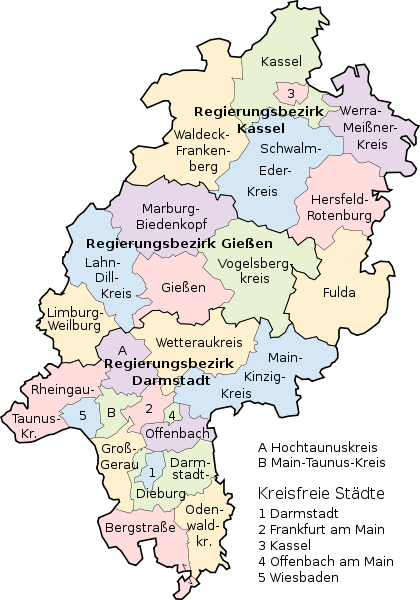
\includegraphics[height=3.5cm]{./images/mesh_orig.png}
				\caption*{Hessen original}
		\end{subfigure}
	\end{figure}
\end{frame}

\begin{frame}
\frametitle{Hessen model} 
	\textbf{Simulation:}\\(with a way to high infection rate)\\
	\hspace{3cm}
	\centering
	\begin{tabular}{c c c c c c }
		0 days
		& 
\includegraphics[height=1.5cm]{./images/0_0S.png}
		& 
\includegraphics[height=1.5cm]{./images/0_1E.png}
		& 
\includegraphics[height=1.5cm]{./images/0_2I.png}
		& 
\includegraphics[height=1.5cm]{./images/0_3R.png}
		& 
\includegraphics[height=1.5cm]{./images/0_4D.png}\\
		9 days
		& 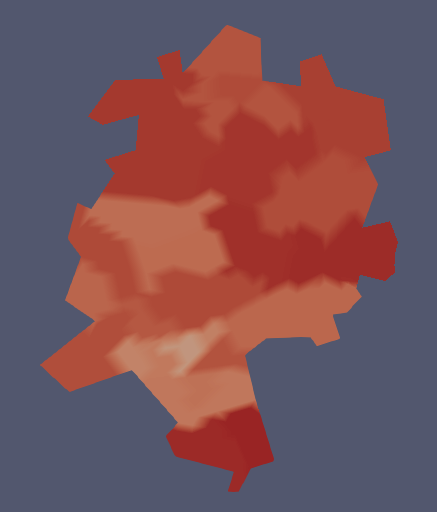
\includegraphics[height=1.5cm]{./images/12_0S.png}
		& 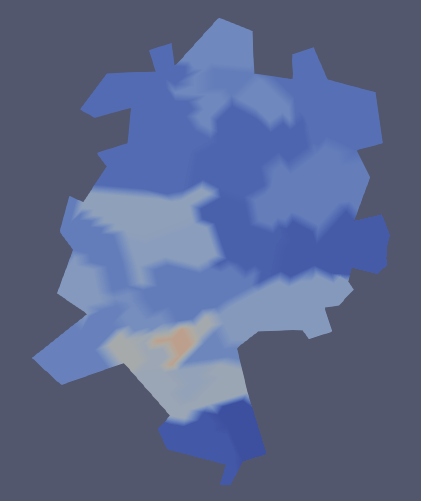
\includegraphics[height=1.5cm]{./images/12_1E.png}
		& 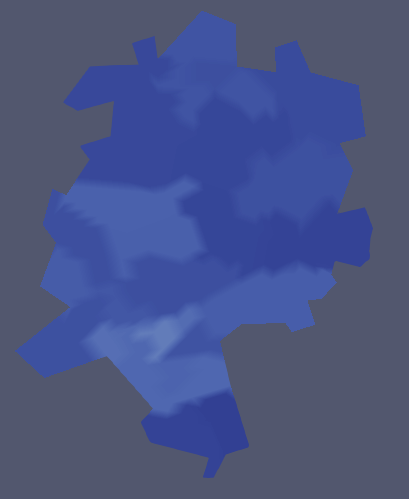
\includegraphics[height=1.5cm]{./images/12_2I.png}
		& 
\includegraphics[height=1.5cm]{./images/12_3R.png}
		& 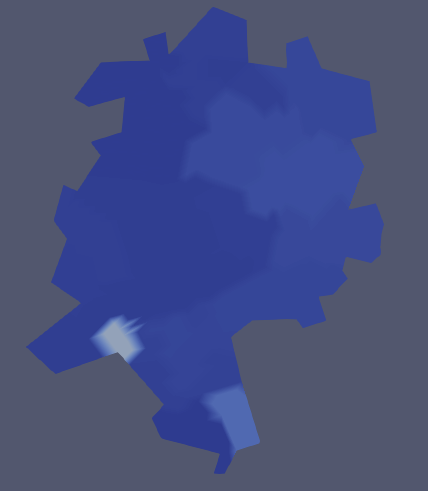
\includegraphics[height=1.5cm]{./images/12_4D.png}\\
		18 days
		& 
\includegraphics[height=1.5cm]{./images/24_0S.png}
		& 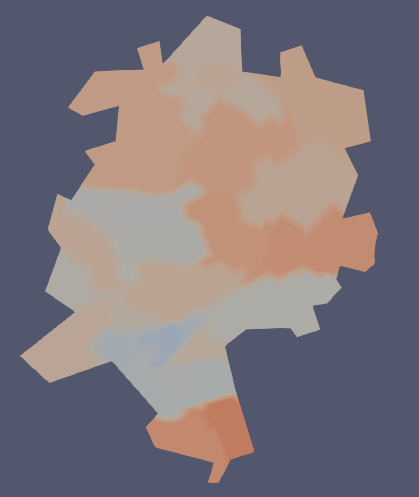
\includegraphics[height=1.5cm]{./images/24_1E.png}
		& 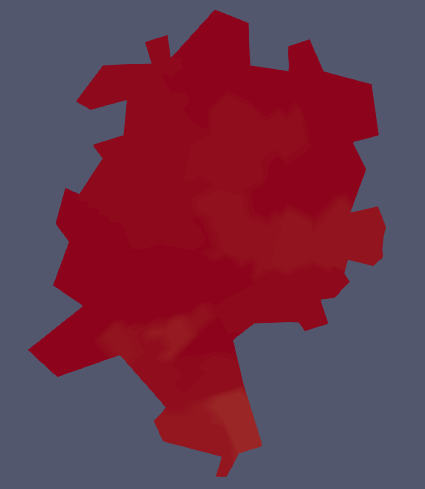
\includegraphics[height=1.5cm]{./images/24_2I.png}
		& 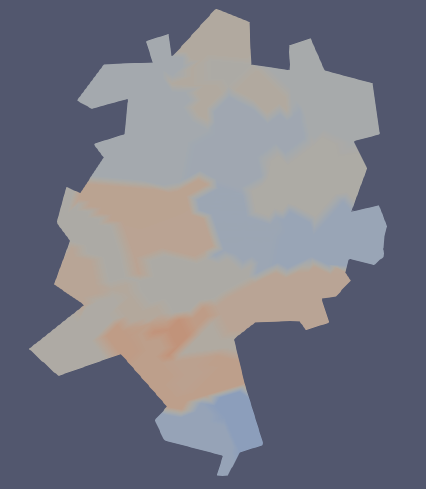
\includegraphics[height=1.5cm]{./images/24_3R.png}
		& 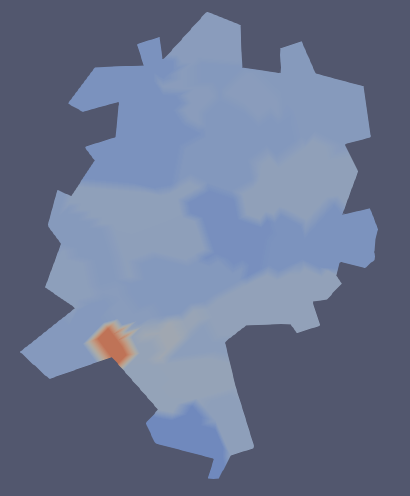
\includegraphics[height=1.5cm]{./images/24_4D.png}\\
		& S & E & I & R & D
	\end{tabular}
\end{frame}
%----------------------------------------------------------------------------------------
\section{Units}
\begin{frame}
	\frametitle{}
\end{frame}

%----------------------------------------------------------------------------------------


\section*{Backup slides}

\begin{frame}
	\frametitle{Math: SEIRD model (ODE)}
	\[
	\begin{array}{ l c c c }
		\text{Susceptibles: }& \frac{dS}{dt} & = & -\alpha SE  \\ \\
		\text{Exposed: }& \frac{dE}{dt} & = & \alpha SE-\frac{1}{qq}E\\ \\
		\text{Infected: }& \frac{dI}{dt} & = & \frac{\kappa}{qq} E-\frac{1}{pp}I\\ \\
		\text{Recovered: }& \frac{dR}{dt} & = & \frac{(1-\kappa)}{qq} E+\frac{(1-\theta)}{pp}I\\ \\
		\text{Diceased: }& \frac{dD}{dt} & = & \frac{\theta}{pp} I \\ \\
	\end{array}	
	\]
\end{frame}

\begin{frame}
	\frametitle{Math: SEIRD model (PDE)} 
	\[
	\begin{array}{ l c c c }
		\text{Susceptibles: }& \frac{d S}{dt} + \nabla[- \text{\textbf{D}} \nabla G] & = & - \alpha SE \\ \\
		\text{Exposed: }& \frac{d E}{dt} + \nabla[- \text{\textbf{D}} \nabla A] & = & (\alpha SE-\frac{1}{qq}E)\\ \\
		\text{Infected: }& \frac{d I}{dt} & = & (\frac{\kappa}{qq} E-\frac{1}{pp}I)\\ \\
		\text{Recovered: }& \frac{d R}{dt} + \nabla[- \text{\textbf{D}} \nabla R]
			& = & (\frac{(1-\kappa)}{qq} E+\frac{(1-\theta)}{pp}I)\\ \\
		\text{Diceased: }& \frac{d D}{dt} & = & \frac{\theta}{pp} I
	\end{array}	
	\]
\end{frame}

\begin{frame}
	\frametitle{Hessen model} 
	\textbf{Current parameters}
	\[
	\begin{array}{ c c c l }
		\alpha & = & 0.800 & \text{(rate of infection)}\\ \\
		\kappa & = & 1.000 & \text{(currently no asympthomaitc cases)}\\ \\
		\theta & = & 0.005 & \text{(0.5\% mortality/infection rate)}\\ \\
		qq & = & 6.000 & \text{(six days until sympthom onset)}\\ \\
		pp & = & 10.000 & \text{(ten days until recovery/death after sympthom onset)}
	\end{array}	
	\]
\end{frame}

\end{document} 
